\documentclass[fontsize=12pt,
               paper=a4,
               twoside=false,
               parskip=half,
               ]{scrartcl}

% Load the packages
% Packages Template
% =================
% 
% Contains packages used for project documentation
% 
% @author burgc5
% 
% To use this simply enter: % Packages Template
% =================
% 
% Contains packages used for project documentation
% 
% @author burgc5
% 
% To use this simply enter: % Packages Template
% =================
% 
% Contains packages used for project documentation
% 
% @author burgc5
% 
% To use this simply enter: \input{./packages.tex}

\usepackage[utf8]{inputenc}
\usepackage[T1]{fontenc}

% Set font to latin modern
\usepackage{lmodern}

\usepackage[pdftex]{graphicx}
\usepackage{epstopdf}

% Create links in pdf documents
\usepackage[colorlinks,pdfpagelabels,pdfstartview=FitH,bookmarksopen=true,bookmarksnumbered=true,linkcolor=black,plainpages=false,hypertexnames=false,citecolor=black] {hyperref}
\hypersetup{
    colorlinks,%
    citecolor=black,%
    filecolor=black,%
    linkcolor=black,%
    urlcolor=black
}
\urlstyle{same}

% Use \enquote{} to create quotation marks
\usepackage{csquotes}

% Create professional tables with booktabs
% @see http://en.wikibooks.org/wiki/LaTeX/Tables#Professional_tables
\usepackage{booktabs}

% Customizable enumerates/itemizes
\usepackage{enumitem}

% SVN meta information
\usepackage{svn}


\usepackage[utf8]{inputenc}
\usepackage[T1]{fontenc}

% Set font to latin modern
\usepackage{lmodern}

\usepackage[pdftex]{graphicx}
\usepackage{epstopdf}

% Create links in pdf documents
\usepackage[colorlinks,pdfpagelabels,pdfstartview=FitH,bookmarksopen=true,bookmarksnumbered=true,linkcolor=black,plainpages=false,hypertexnames=false,citecolor=black] {hyperref}
\hypersetup{
    colorlinks,%
    citecolor=black,%
    filecolor=black,%
    linkcolor=black,%
    urlcolor=black
}
\urlstyle{same}

% Use \enquote{} to create quotation marks
\usepackage{csquotes}

% Create professional tables with booktabs
% @see http://en.wikibooks.org/wiki/LaTeX/Tables#Professional_tables
\usepackage{booktabs}

% Customizable enumerates/itemizes
\usepackage{enumitem}

% SVN meta information
\usepackage{svn}


\usepackage[utf8]{inputenc}
\usepackage[T1]{fontenc}

% Set font to latin modern
\usepackage{lmodern}

\usepackage[pdftex]{graphicx}
\usepackage{epstopdf}

% Create links in pdf documents
\usepackage[colorlinks,pdfpagelabels,pdfstartview=FitH,bookmarksopen=true,bookmarksnumbered=true,linkcolor=black,plainpages=false,hypertexnames=false,citecolor=black] {hyperref}
\hypersetup{
    colorlinks,%
    citecolor=black,%
    filecolor=black,%
    linkcolor=black,%
    urlcolor=black
}
\urlstyle{same}

% Use \enquote{} to create quotation marks
\usepackage{csquotes}

% Create professional tables with booktabs
% @see http://en.wikibooks.org/wiki/LaTeX/Tables#Professional_tables
\usepackage{booktabs}

% Customizable enumerates/itemizes
\usepackage{enumitem}

% SVN meta information
\usepackage{svn}


% SVN Meta
\SVN $Date: 2012-05-04 16:15:57 +0200 (Fr, 04 Mai 2012) $
\SVN $Revision: 98 $
\SVN $HeadURL: https://svn.bfh.ch/repos/projects/patmon1/trunk/doc/src/domain_model.tex $


\begin{document}

% Document title for title.tex
\newcommand{\doctitle}{Domain Model}
\newcommand{\docrevision}{68}
% Titlepage Template
% ==================
% 
% @author burgc5
% 
% To use this simply enter: % Titlepage Template
% ==================
% 
% @author burgc5
% 
% To use this simply enter: % Titlepage Template
% ==================
% 
% @author burgc5
% 
% To use this simply enter: \input{./title.tex}
% 
% You have to define the commands '\doctitle' and '\docrevision' to give the 
% document a title and a revision on its titlepage.
% Do this with the following command:
% \newcommand{\doctitle}{Document title goes here}
%
% SVN:
% ----
% You also have to define the variables:
% \SVN $Date$
% \SVN $Revision$
%
% As executing the following command on the file:
% > svn propset svn:keywords "Date Revision" filename.tex
% 
% This titlepage needs:
% \usepackage[pdftex]{graphicx}
% \usepackage{svn}
%

\begin{titlepage}

\begin{center}

% Team-logo

\includegraphics[width=0.35\textwidth]{./comet-logo.eps}\\[2.5cm]    

% Project title
\textsc{\Large Comet Patient Monitor}\\[2cm]

% Document title
{ \huge \bfseries \doctitle{}}\\[3cm]

% Members/Client
\begin{minipage}{0.45\textwidth}
\begin{flushleft} \large
\emph{Team Members:}\\
Patrick \textsc{Haring}\\
Christian \textsc{Bürgi}
\end{flushleft}
\end{minipage}
\begin{minipage}{0.45\textwidth}
\begin{flushright} \large
\emph{Client:} \\
Prof.~Dr.~Olivier \textsc{Biberstein}\\
~
\end{flushright}
\end{minipage}

\vfill

{\large 
Revision: \SVNRevision \\[0.2cm]
\SVNDate \\[0.2cm]
{\footnotesize \itshape \url{\SVNHeadURL?p=\SVNRevision}}}

\end{center}

\end{titlepage}
% 
% You have to define the commands '\doctitle' and '\docrevision' to give the 
% document a title and a revision on its titlepage.
% Do this with the following command:
% \newcommand{\doctitle}{Document title goes here}
%
% SVN:
% ----
% You also have to define the variables:
% \SVN $Date$
% \SVN $Revision$
%
% As executing the following command on the file:
% > svn propset svn:keywords "Date Revision" filename.tex
% 
% This titlepage needs:
% \usepackage[pdftex]{graphicx}
% \usepackage{svn}
%

\begin{titlepage}

\begin{center}

% Team-logo

\includegraphics[width=0.35\textwidth]{./comet-logo.eps}\\[2.5cm]    

% Project title
\textsc{\Large Comet Patient Monitor}\\[2cm]

% Document title
{ \huge \bfseries \doctitle{}}\\[3cm]

% Members/Client
\begin{minipage}{0.45\textwidth}
\begin{flushleft} \large
\emph{Team Members:}\\
Patrick \textsc{Haring}\\
Christian \textsc{Bürgi}
\end{flushleft}
\end{minipage}
\begin{minipage}{0.45\textwidth}
\begin{flushright} \large
\emph{Client:} \\
Prof.~Dr.~Olivier \textsc{Biberstein}\\
~
\end{flushright}
\end{minipage}

\vfill

{\large 
Revision: \SVNRevision \\[0.2cm]
\SVNDate \\[0.2cm]
{\footnotesize \itshape \url{\SVNHeadURL?p=\SVNRevision}}}

\end{center}

\end{titlepage}
% 
% You have to define the commands '\doctitle' and '\docrevision' to give the 
% document a title and a revision on its titlepage.
% Do this with the following command:
% \newcommand{\doctitle}{Document title goes here}
%
% SVN:
% ----
% You also have to define the variables:
% \SVN $Date$
% \SVN $Revision$
%
% As executing the following command on the file:
% > svn propset svn:keywords "Date Revision" filename.tex
% 
% This titlepage needs:
% \usepackage[pdftex]{graphicx}
% \usepackage{svn}
%

\begin{titlepage}

\begin{center}

% Team-logo

\includegraphics[width=0.35\textwidth]{./comet-logo.eps}\\[2.5cm]    

% Project title
\textsc{\Large Comet Patient Monitor}\\[2cm]

% Document title
{ \huge \bfseries \doctitle{}}\\[3cm]

% Members/Client
\begin{minipage}{0.45\textwidth}
\begin{flushleft} \large
\emph{Team Members:}\\
Patrick \textsc{Haring}\\
Christian \textsc{Bürgi}
\end{flushleft}
\end{minipage}
\begin{minipage}{0.45\textwidth}
\begin{flushright} \large
\emph{Client:} \\
Prof.~Dr.~Olivier \textsc{Biberstein}\\
~
\end{flushright}
\end{minipage}

\vfill

{\large 
Revision: \SVNRevision \\[0.2cm]
\SVNDate \\[0.2cm]
{\footnotesize \itshape \url{\SVNHeadURL?p=\SVNRevision}}}

\end{center}

\end{titlepage}

\tableofcontents

\section{Domain Model}

% Diagram generated with astah
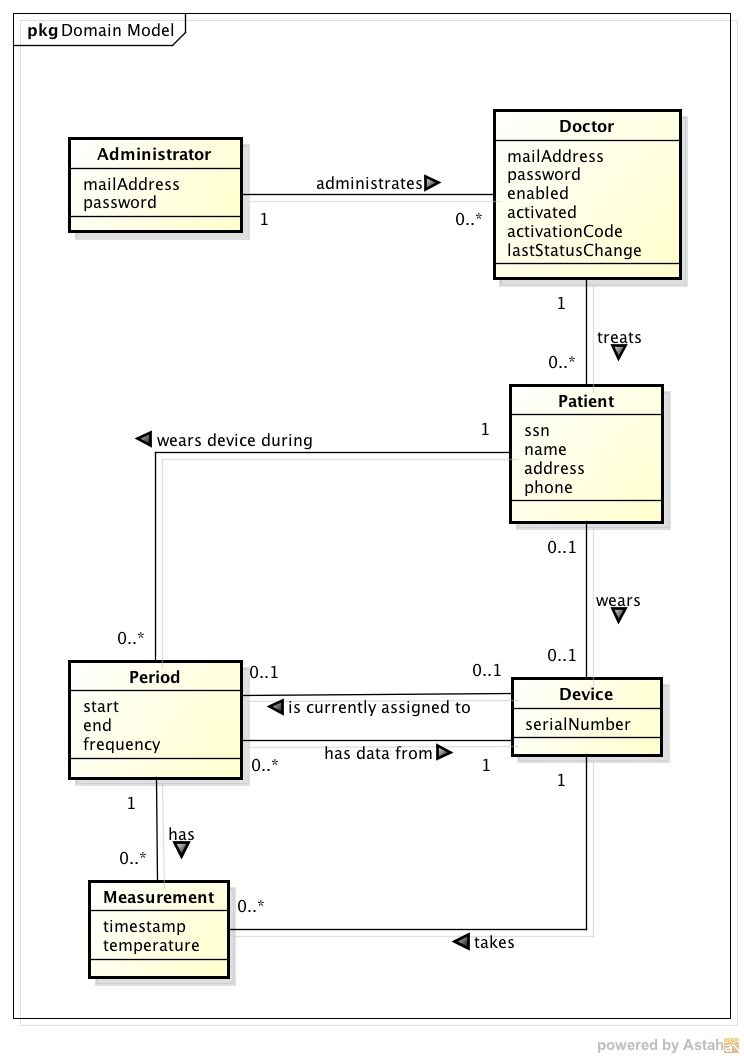
\includegraphics[width=14cm]{./domain-model.png}

\section{Description}

\subsection{Classes}

\subsubsection{Administrator} 

The \texttt{Administrator} has the attributes \texttt{mailAddress} and \texttt{password} which are used as credentials to authenticate against the system. 

\subsubsection{Doctor}
Each \texttt{Doctor} has an email address and a password. They are stored in the attributes \texttt{mailAddress} and \texttt{password}, which are used as credentials to authenticate against the system. \texttt{Enabled} indicates wether the account is enabled oder disabled. The attributes \texttt{activated} and \texttt{activationCode} are used for the activation process. \texttt{Activated} indicates whether the \texttt{Doctor} is activated or not, \texttt{activationCode} stores the activation code which was sent to him by email. For a successful login into the system, both \texttt{enabled} and \texttt{activated} have to be true. In order to delete an account, it has to be disabled for a given time period. Therefore a timestamp called \texttt{lastStatusChange} shows when the last status change occurred. A status change is either a change of \texttt{enabled} or \texttt{activated}.

\subsubsection{Patient}
Each \texttt{Patient} is identified by his social security number (SSN) which is stored the attribute \texttt{ssn}. The attributes \texttt{name}, \texttt{address} and \texttt{phone} are mandatory and will help the \texttt{Doctor} to identify the \texttt{Patient}. 

\subsubsection{Period}
The class \texttt{Period} represents a monitoring period during which a \texttt{Device} is monitoring data on a \texttt{Patient}. The attributes \texttt{start} and \texttt{end} represent the interval of time and the attribute \texttt{frequency} represents the frequency by which the \texttt{Measurement}s are taken.

\subsubsection{Device}
Each \texttt{Device} is identified by its serial number, which is stored in the attribute \texttt{serialNumber}.

\subsubsection{Measurement}
The class \texttt{Measurement} represents the \texttt{temperature} which was taken by a \texttt{Device} at a given time \texttt{timestamp}.


\subsection{Relationships}


\subsubsection{Administrator administrates Doctor}

The \texttt{Administrator} can have zero to n \texttt{Doctor}s he administrates in the system. In the initial state of the system, there is no \texttt{Doctor}. As the system should be able to handle a big amount of \texttt{Doctor}s, they are all related to the \texttt{Administrator} they were created by.


\subsubsection{Doctor treats Patient}

\texttt{Doctor}s treat from zero to n \texttt{Patient}s. When a \texttt{Doctor} is created, he doesn't treat any \texttt{Patient}. When doing treatments, he gets assigned all \texttt{Patient}s he treats. On the other side, \texttt{Patient}s can only be treated by a single \texttt{Doctor} (and there has to be a \texttt{Doctor} who treats the \texttt{Patient}).


\subsubsection{Patient wears Device}

When a \texttt{Device} is assigned to a \texttt{Patient}, this relationship represents that a specific \texttt{Device} is actually worn by a specific \texttt{Patient}. A \texttt{Device} can only be worn by a single \texttt{Patient} at the same time. On the other hand, a \texttt{Patient} can only wear a single \texttt{Device} at the same time. This relationship can also be represented by \enquote{\texttt{Patient} wears device during \texttt{Period}} and \enquote{\texttt{Device} is currently assigned to \texttt{Period}}. Therefore it is intended that this relationship is not implemented in the actual code.


\subsubsection{Patient wears device during Period}

\texttt{Patient}s which are monitored need to have assigned a \texttt{Period} in which the monitoring takes place. \texttt{Patient}s can have multiple \texttt{Period}s if they are treated more than once, but a \texttt{Period} can only belong to a single \texttt{Patient} and the \texttt{Period} has to belong to a \texttt{Patient}.


\subsubsection{Period has data from Device}

In order to detect which \texttt{Device} records or has recorded the \texttt{Period}'s date, there is a relationship between \texttt{Period} and \texttt{Device}. \texttt{Period}s have exactly one \texttt{Device} since there is only one \texttt{Device} recording data for it. On the other hand, \texttt{Device}s can record data for any number of \texttt{Period}s, since they can be reconfigured to a new \texttt{Period} after they have completed monitoring for an arbitrary \texttt{Period}. The condition, that a \texttt{Device} can only be configured for a single \texttt{Period} at a time, is not directly represented in the model and has to be checked programmatically. This is done using the relationship \enquote{\texttt{Device} is currently assigned to \texttt{Period}}.


\subsubsection{Device is currently assigned to Period}

\texttt{Period}s have a second relationship to \texttt{Device}. This relationship shows, that the \texttt{Device} is configured for the \texttt{Period}. A \texttt{Device} can only be assigned to one \texttt{Period} at a time. The \texttt{Period} which the \texttt{Device} is configured to must be the same as in the relationship \enquote{\texttt{Period} has data from \texttt{Device}}.


\subsubsection{Period has Measurement}

\texttt{Period}s have a relationship to \texttt{Measurement} showing which \texttt{Measurement} has been taken for which \texttt{Period}. \texttt{Measurement}s belong to exactly one \texttt{Period} but a \texttt{Period} can have any number of \texttt{Measurement}s (including none).


\subsubsection{Device takes Measurement}

\texttt{Measurement}s are taken by \texttt{Device}s. They belong exactly to one \texttt{Device}. On the other hand, \texttt{Devices} can take any number of \texttt{Measurement}s. This relationship can be reflected using \enquote{\texttt{Period} has data from \texttt{Device}} and \enquote{\texttt{Period} has \texttt{Measurement}}. Therefore it is intended that this relationship is not implemented in the actual code.

\end{document}